\chapter{Introduction}
\label{ch:Intro}


%%%%%%%%%%%%%%%%%%%%%%%%%%%%%%%%%%%%%%%%%%%%%%%%%%
\section{Functional genomics and gene regulation}
%
\section{Genetic variation and disease}
Understanding the genetic variation underlying disease susceptibility and aetiology may contribute to better diagnosis, treatment and prevention of disease. In general, GWAS have limited value in terms of risk prediction but are important for the discovery of new genes and pathways involved in disease pathogenesis and potential drug targets \parencite{Kooperberg2010}.
%%%

\subsection*{\textit{Cis} and \textit{trans} eQTL}
SNPs with an eQTL association can be classified as either \textit{cis} or \textit{trans} acting depending on the distance between the SNP and gene of interest. Although somewhat arbitrary, \textit{cis} acting variants generally reside 250kb-1Mb from the gene. \textit{Trans} SNPs are located elsewhere in the genome, including other chromosomes (Figure~\ref{fig:intro.eQTL}) \parencite{Williams2010}.  \textit{Cis} acting eQTL tend to be enriched around the transcription start site of the gene and occur more frequently in exonic regions \parencite{Veyrieras2008, Nica2011}. \textit{Trans} effects are often weaker but may involve master regulators: factors that have multiple effects on gene expression \parencite{Morley2004}. \textit{Trans} SNPs may exert their effects through transcript stability as well as transcript production for example through protein-RNA interactions or small interfering RNAs (siRNAs) \parencite{Grosshans2008}.

\begin{figure}[H]
\includegraphics[width=\textwidth]{./Introduction/eQTL.pdf}%
\caption[Effect of regulatory variants on expression levels of genes]{\textbf{Effect of regulatory variants on expression levels of genes}. Reprinted by permission from Macmillan Publishers Ltd: Nature Reviews Genetics \parencite{Cheung2009}, copyright 2009. The effect of local (\textit{cis}) or distal (\textit{trans}) regulatory variants on levels of gene expression.}%
\label{fig:intro.eQTL}%
\end{figure}


\section{Sepsis}
Sepsis is defined as the systemic inflammatory response to the presence of an infection and is classified as severe when associated with organ dysfunction, hypoperfusion abnormality or sepsis-induced hypotension.  Systemic inflammatory response syndrome (SIRS) is used to describe the inflammatory response and it includes at least two of the clinical manifestations detailed in Table \ref{tab:SIRS.sepsis} \parencite{Bone1992}.  However this definition is limited in that the microbiological basis of the response is not considered and there is no graduation of severity.  In the UK, severe sepsis accounts for 27\% of ICU admissions \parencite{Padkin2003} and from a number of studies in both the UK and America, mortality has been estimated to be between 28\% and 50\% \parencite{Angus2001, Padkin2003, Sands1997, Zeni1997}. \\
%\ToDo{Table 1.2 in Jay't thesis, revised criteria in 2001?}.

\begin{table}[H]
\centering\doublespacing
\caption[The clinical manifestations of SIRS]{\textbf{The clinical manifestations of SIRS \parencite{Bone1992}.} SIRS is diagnosed in patients with at least two of these clinical manifestations.}  
\label{tab:SIRS.sepsis}
\begin{tabular}{>{\centering\arraybackslash}m{0.9\textwidth}}
\\ \toprule
\textbf{SIRS clinical manifestations} \\ 
\midrule
Body temperature \textgreater 38\degree C \\
Heart rate \textgreater 90 beats per minute \\
Respiratory rate \textgreater 20 breaths per minute or hyperventilation \newline as indicated by a PACO\textsubscript{2} of \textless 32 mm Hg \\
An alteration in the white blood cell count (count \textgreater 12,000/cu mm or \newline \textless 400/cu mm or the presence of \textgreater 10\% immature neutrophils)\\
\bottomrule
\end{tabular}
\end{table}



%%%%%%%%%%%%%%%%%%%%%%%%%%%%%%%
\section{Common variable immune deficiency disorders}

Primary immunodeficiencies (PIDs) are a group of rare disorders that result from a failure in the immune system and CVID are the most frequently encountered PID in the clinic \parencite{Park2008}. CVID are a group of diseases in which insufficient quantity and quality of immunoglobulin usually leads to susceptibility to recurrent bacterial infections, mainly of the respiratory and gastrointestinal tracts \parencite{Chapel2009}.  An immunodeficiency is recognized in most CVID patients in the second, third or fourth decade of life and the first diagnostic criteria were published in 1999 (Table~\ref{tab:criteria.cvid}) \parencite{Conley1999}.  These criteria have been used since then with slight variations for example, the minimum age of presentation is often increased to 4 years in order to avoid infants with immune defects which cause B cell differentiation and class-switch disorders \parencite{Chapel2008}.

\begin{table}[H]
\centering
\singlespacing
\caption[CVID diagnosis criteria]{\textbf{CVID diagnosis criteria.} Individuals fulfilling each of the criteria are diagnosed with CVID \parencite{Conley1999}. SD = standard deviations.}  
\label{tab:criteria.cvid}
\begin{tabular}{c}
\toprule
\textbf{Criteria for CVID diagnosis} \\ 
\midrule
Male or female patient \textgreater 2 years of age\\
Serum IgG and IgA at least 2 SD below the mean for age \\
IgM is present or absent\\
Poor response to vaccines \\
Absent isohemagglutinins \\
Defined causes of hypogammaglobulinemia have been excluded \\
Normal or low B cell numbers \\
\bottomrule
\end{tabular}
\end{table} 

%%%
\subsection{Clinical complications}
The diagnosis of CVID is made by excluding known disorders of B cell failure for example B cell differentiation defects resulting in absent B cells, activation-induced cytidine deaminase (AID) and uracil-DNA glycosylase (UNG) deficiencies affecting B cell function and T cell switching pathways \parencite{Chapel2008}. This results in a heterogeneous group of individuals with widely different clinical features and additional complications.

Within cohorts of CVID patients, beyond bacterial infections, the main clinical complications observed include autoimmunity, lymphocytic infiltration, enteropathy and malignancy (Figure~\ref{fig:complications.intro.cvid}). Patients with at least one clinical complication have a much poorer survival rate compared to those with an Infections Only phenotype \parencite{Chapel2008}.

\begin{figure}[H]
\centering
\begin{subfigure}[b]{0.49\textwidth}
	\centering
	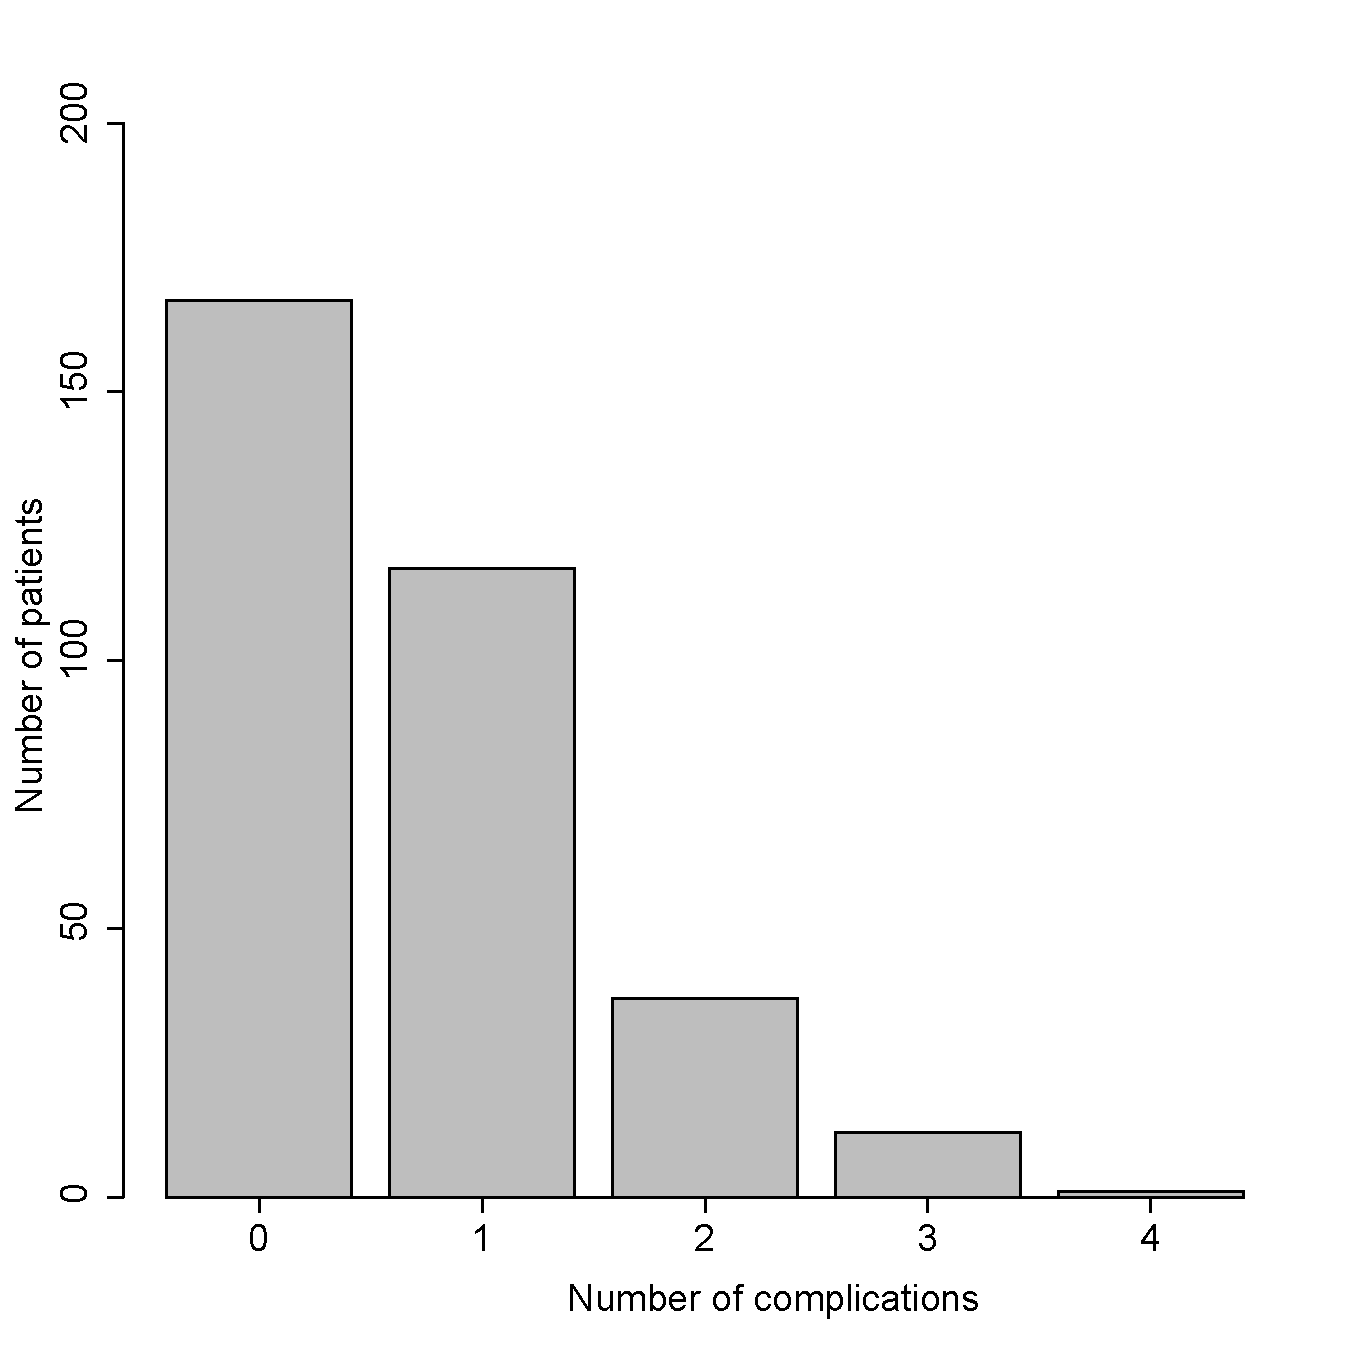
\includegraphics[width=\textwidth]{./Introduction/Barplot_complications_cvid.pdf}%
	\caption{Number of complications}%
\end{subfigure}
\begin{subfigure}[b]{0.49\textwidth}
	\centering
	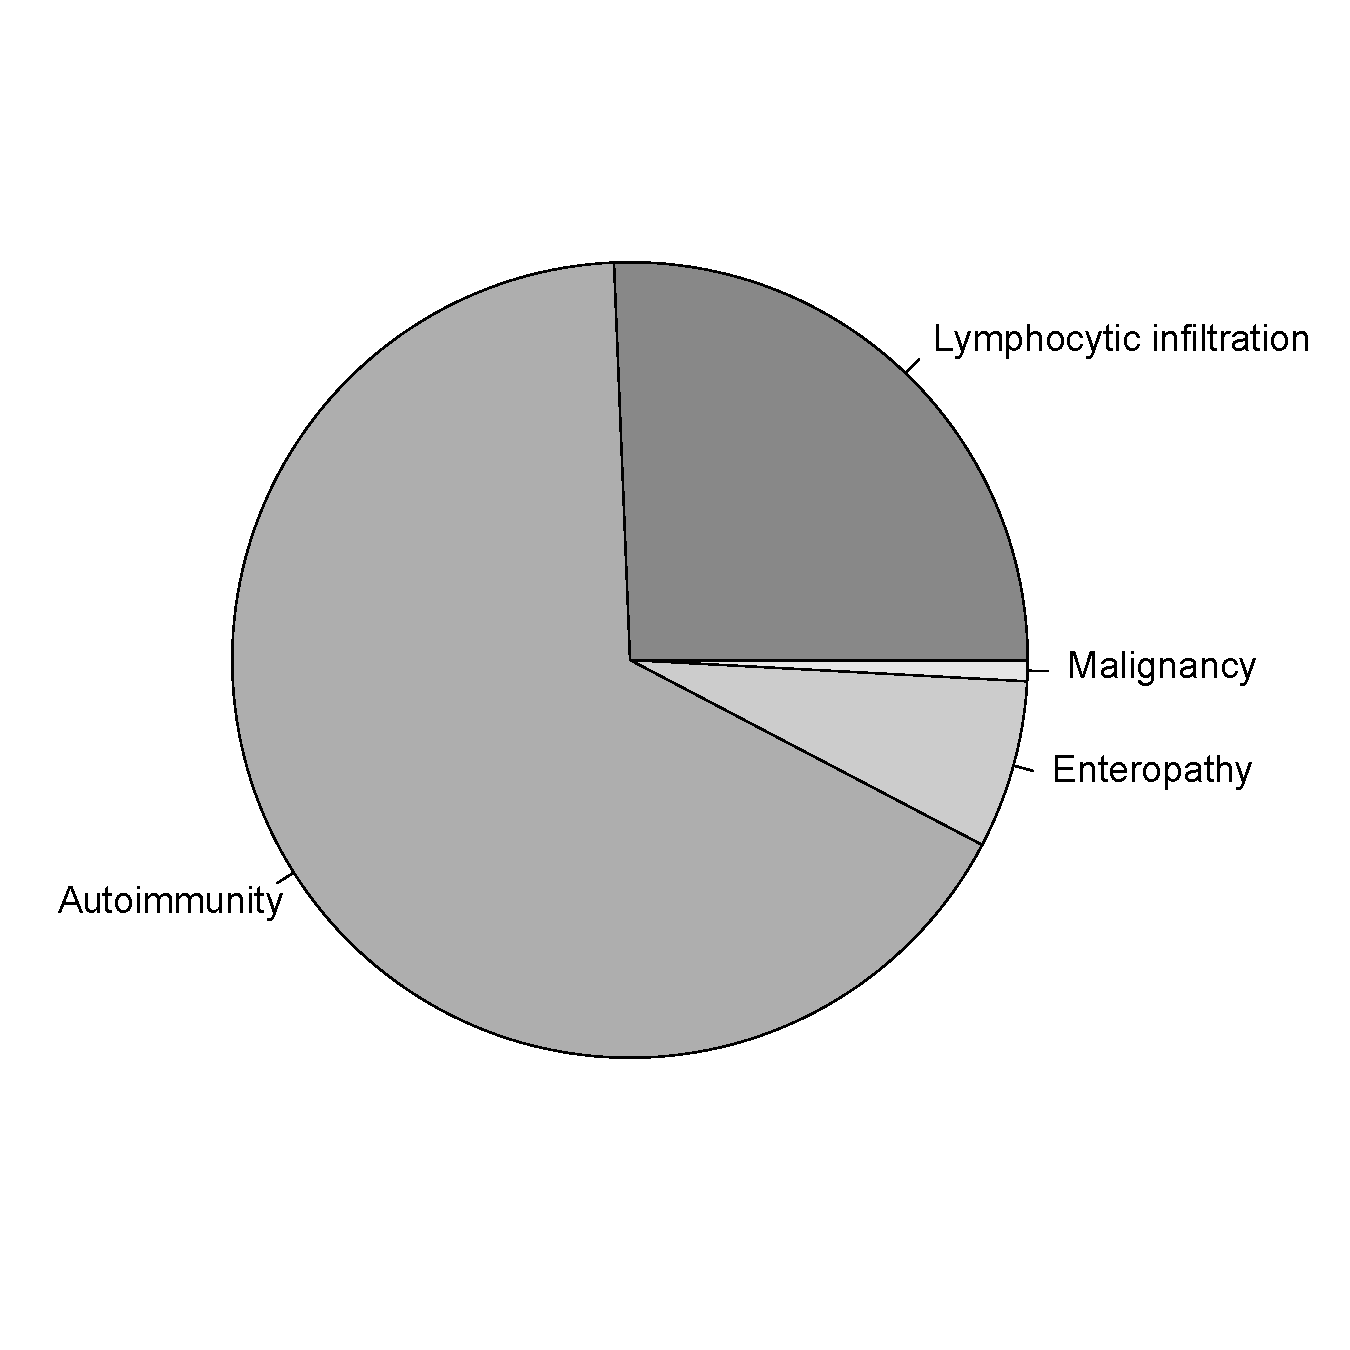
\includegraphics[width=\textwidth]{./Introduction/Pie_1complication.pdf}%
	\caption{One complication}%
\end{subfigure}
\begin{subfigure}[b]{0.49\textwidth}
	\centering
	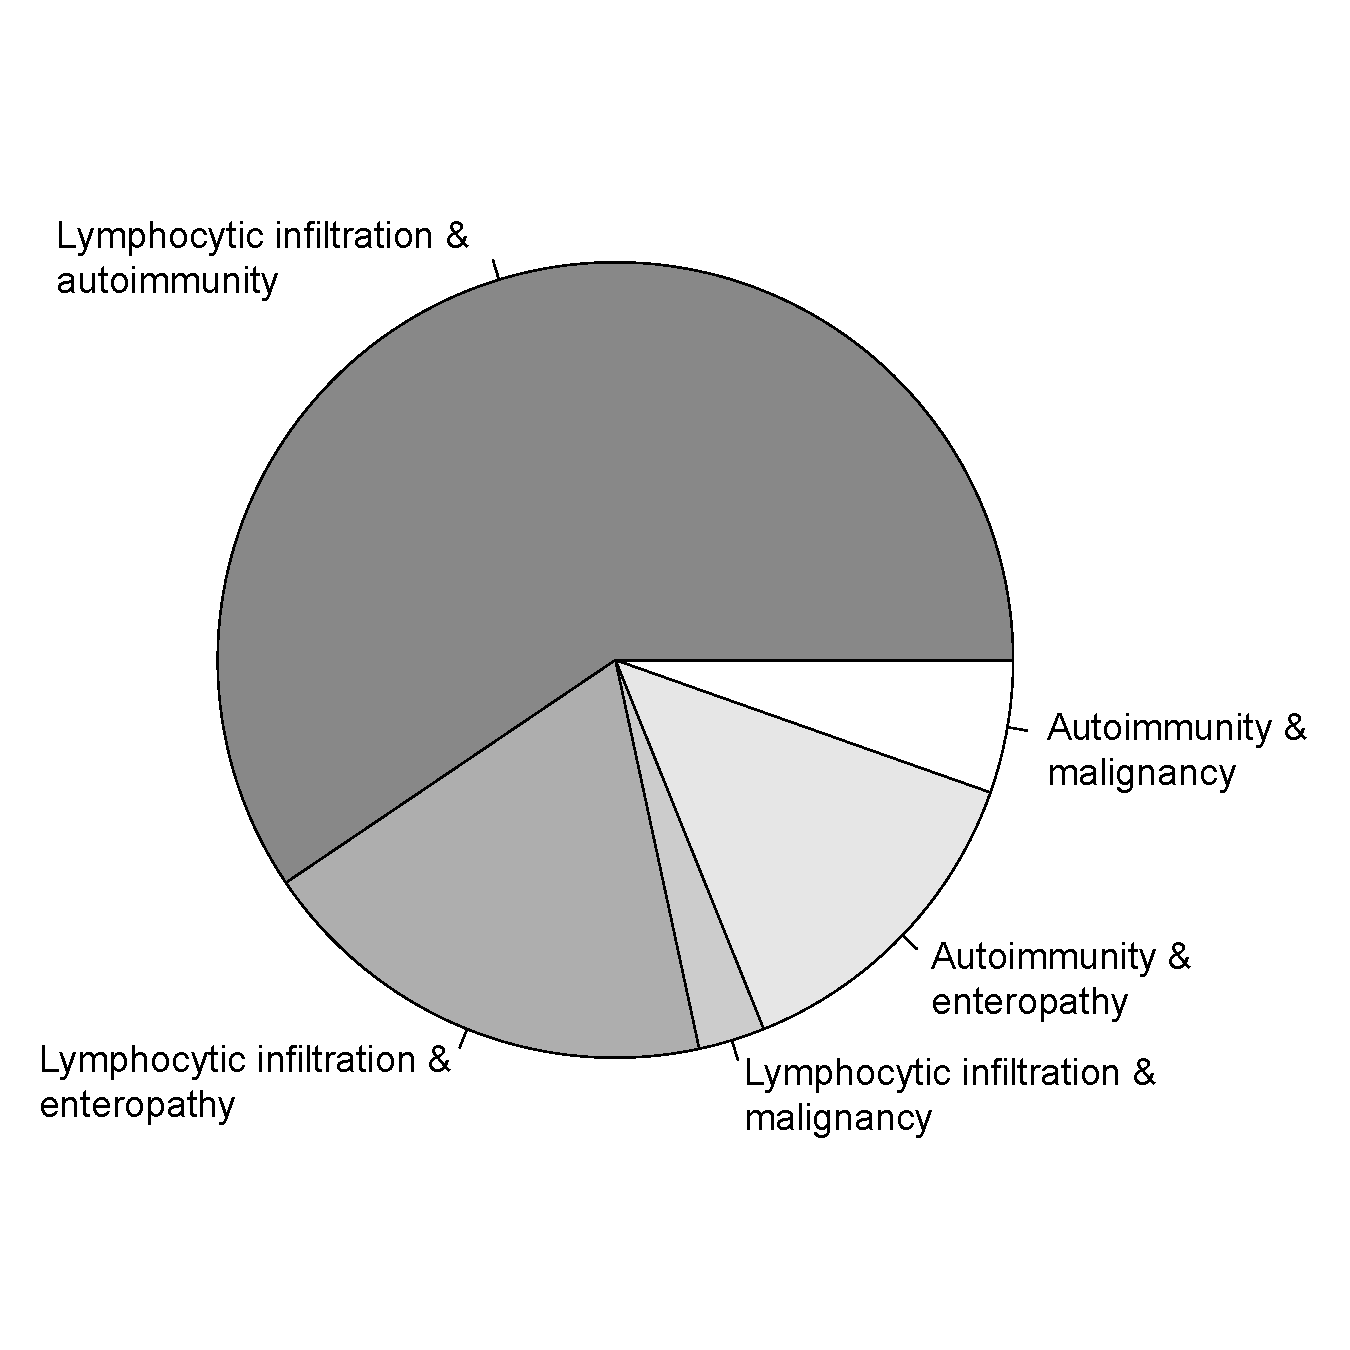
\includegraphics[width=\textwidth]{./Introduction/Pie_2complication.pdf}%
	\caption{Two complications}%
\end{subfigure}
\begin{subfigure}[b]{0.49\textwidth}
	\centering
	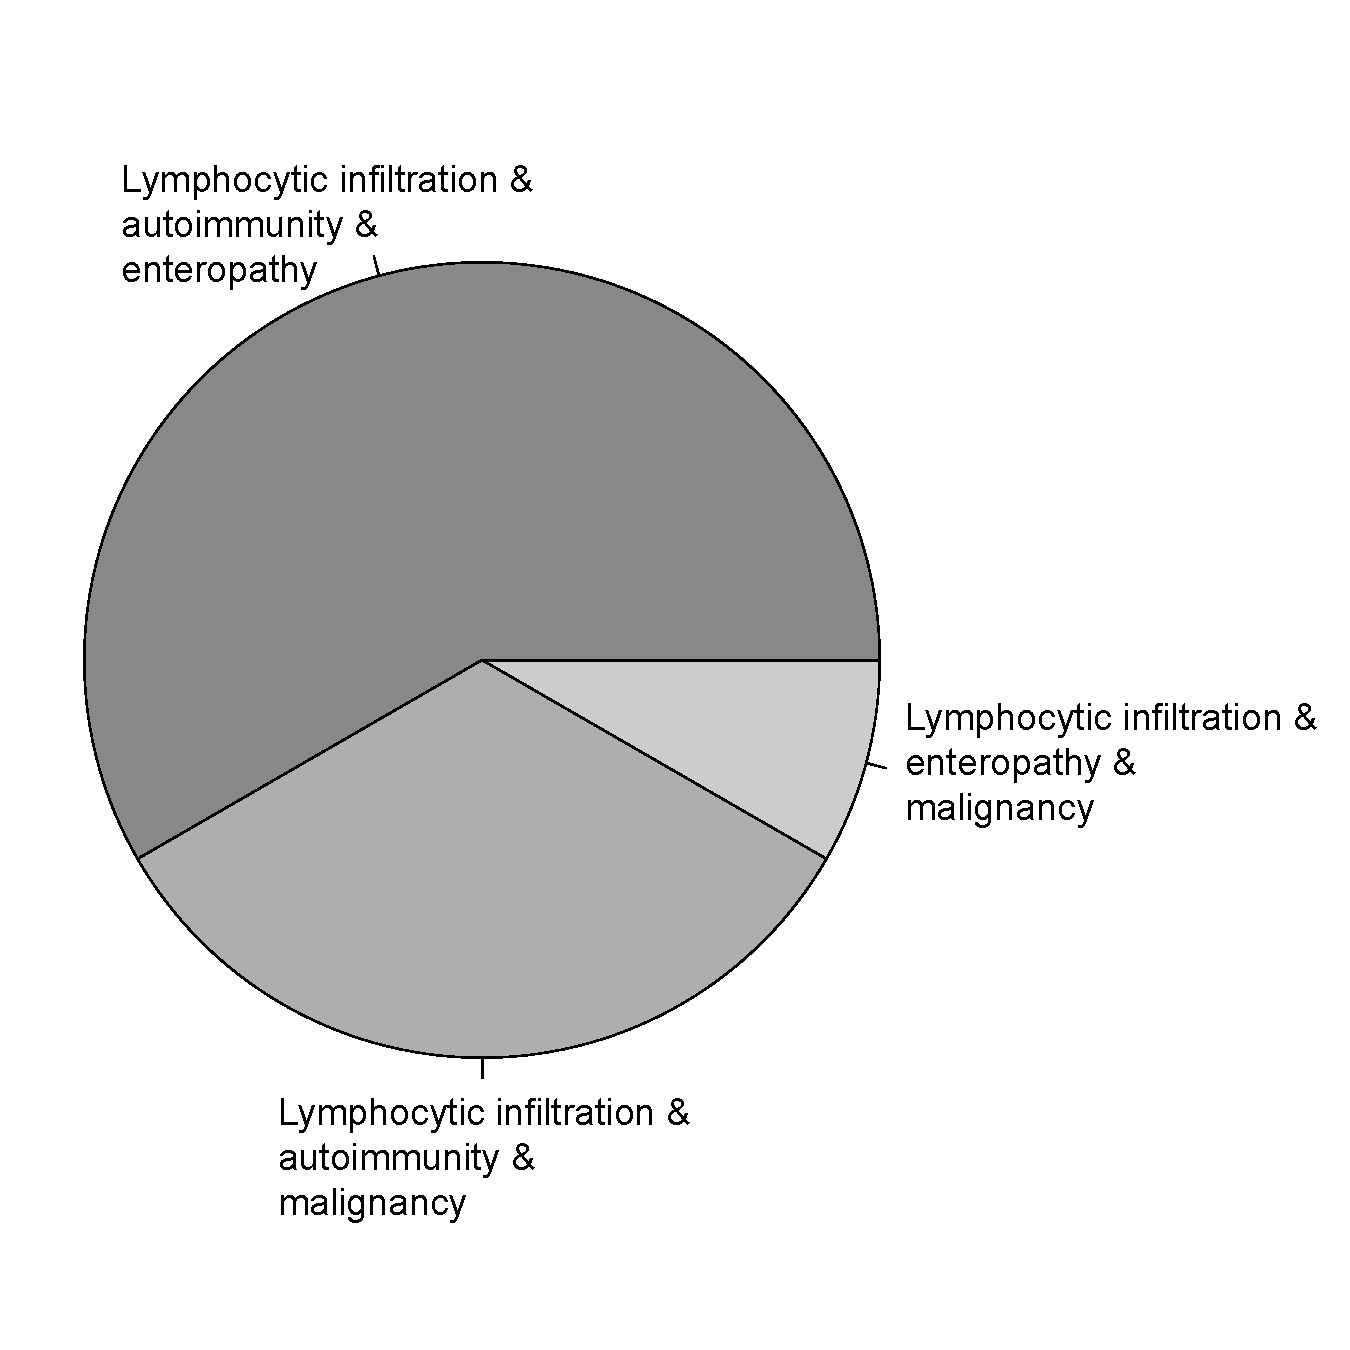
\includegraphics[width=\textwidth]{./Introduction/Pie_3complication.pdf}%
	\caption{Three complications}%
\end{subfigure}
\caption[Nature and number of CVID complications]{\textbf{Nature and number of CVID complications.} a) Number of complications observed in each individual. Individuals with no complications are referred to as infections only. b) Distribution of complications in patients with one complication. c)  Distribution of complications in patients with two complications. d)  Distribution of complications in patients with three complications. \parencite{Chapel2008}}
\label{fig:complications.intro.cvid}
\end{figure}


